\documentclass[tikz,border=2pt]{standalone}
\usepackage{tikz}
\usepackage{pgfplots}
\pgfplotsset{compat=1.16}
\usetikzlibrary{shapes.geometric,shapes.multipart,positioning,arrows,arrows.meta,calc,chains,decorations.pathreplacing,backgrounds}
\usepackage{xcolor}
\begin{document}
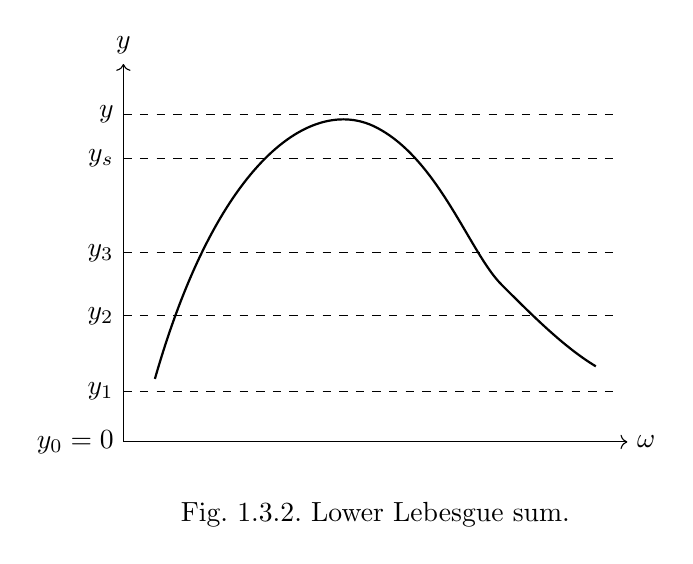
\begin{tikzpicture}[scale=0.8]
    % Axes
    \draw[->] (0,0) -- (8,0) node[right] {$\omega$};
    \draw[->] (0,0) -- (0,6) node[above] {$y$};

    % Curve (representing X(omega))
    \draw[thick] (0.5,1) .. controls (1.5,4.5) and (3,5.5) .. (4,5)
                 .. controls (5,4.5) and (5.5,3) .. (6,2.5)
                 .. controls (6.5,2) and (7,1.5) .. (7.5,1.2);

    % Horizontal dashed lines for y levels
    \draw[dashed] (0,0.8) -- (7.8,0.8);
    \draw[dashed] (0,2) -- (7.8,2);
    \draw[dashed] (0,3) -- (7.8,3);
    \draw[dashed] (0,4.5) -- (7.8,4.5);
    \draw[dashed] (0,5.2) -- (7.8,5.2);

    % Y-axis labels
    \node[left] at (0,0) {$y_0 = 0$};
    \node[left] at (0,0.8) {$y_1$};
    \node[left] at (0,2) {$y_2$};
    \node[left] at (0,3) {$y_3$};
    \node[left] at (0,4.5) {$y_s$};
    \node[left] at (0,5.2) {$y$};

    % Caption
    \node[below] at (4,-0.8) {Fig.\ 1.3.2.\ Lower Lebesgue sum.};
\end{tikzpicture}
\end{document}
